\subsection{Adding Functional Reactive Programming}
\label{sec:step2_frp}
As shown in the first step, the need to handle $\Delta t$ explicitly can be quite messy, is inelegant and a potential source of errors, also the explicit handling of the state of an agent and its behavioural function is not very modular. We can solve both these weaknesses by switching to the functional reactive programming paradigm (FRP), because it allows to express systems with discrete and continuous time-semantics.

In this step we are focusing on Arrowized FRP \cite{hughes_generalising_2000} using the library Yampa \cite{hudak_arrows_2003}. In it, time is handled implicit, meaning it cannot be messed with, which is achieved by building the  whole system on the concept of signal functions (SF). An SF can be understood as a process over time and is technically a continuation which allows to capture state using closures. Both these fundamental features allow us to tackle the weaknesses of our first step and push our approach further towards a truly elegant functional approach.

\subsubsection{Implementation}
We start by defining an agent now as an SF which receives the states of all agents as input and outputs the state of the agent:

\begin{HaskellCode}
type SIRAgent = SF [SIRState] SIRState 
\end{HaskellCode}

Now we can define the behaviour of an agent to be the following:

\begin{HaskellCode}
sirAgent :: RandomGen g => g -> SIRState -> SIRAgent
sirAgent g Susceptible = susceptibleAgent g
sirAgent g Infected    = infectedAgent g
sirAgent _ Recovered   = recoveredAgent
\end{HaskellCode}

Depending on the initial state we return the corresponding behaviour. Most notably is the difference that we are now passing a random-number generator instead of running in the Random Monad because signal functions as implemented in Yampa are not capable of being monadic. We see that the recovered agent ignores the random-number generator which is in accordance with the implementation in the previous step where it acts as a sink which returns constantly the same state:

\begin{HaskellCode}
recoveredAgent :: SIRAgent
recoveredAgent = arr (const Recovered)
\end{HaskellCode}

When an event occurs we can change the behaviour of an agent using the Yampa combinator \textit{switch}, which is much more elegant and expressive than the initial approach as it makes the change of behaviour at the occurrence of an event explicit. Thus a susceptible agent behaves as susceptible until it becomes infected. Upon infection an \textit{Event} is returned which results in switching into the \textit{infectedAgent} SF, which causes the agent to behave as an infected agent from that moment on. Instead of randomly drawing the number of contacts to make, we now follow a fundamentally different approach by using Yampas \textit{occasionally} function. This requires us to carefully select the right $\Delta t$ for sampling the system as will be shown in results. 

%\begin{samepage}
\begin{HaskellCode}
susceptibleAgent :: RandomGen g => g -> SIRAgent
susceptibleAgent g = 
    switch (susceptible g) (const (infectedAgent g))
  where
    susceptible :: RandomGen g 
      => g -> SF [SIRState] (SIRState, Event ())
    susceptible g = proc as -> do
      makeContact <- occasionally g (1 / contactRate) () -< ()
      if isEvent makeContact
        then (do
          a <- drawRandomElemSF g -< as
          case a of
            Infected -> do
              i <- randomBoolSF g infectivity -< ()
              if i
                then returnA -< (Infected, Event ())
                else returnA -< (Susceptible, NoEvent)
             _       -> returnA -< (Susceptible, NoEvent))
        else returnA -< (Susceptible, NoEvent)
\end{HaskellCode}
%\end{samepage}

We deal with randomness different now and implement signal functions built on the \textit{noiseR} function provided by Yampa. This is an example for the stream character and statefulness of a signal function as it needs to keep track of the changed random-number generator internally through the use of continuations and closures. Here we provide the implementation of \textit{randomBoolSF}, \textit{drawRandomElemSF} works similar but takes a list as input and returns a randomly chosen element from it:

\begin{HaskellCode}
randomBoolSF :: RandomGen g => g -> Double -> SF () Bool
randomBoolSF g p = proc _ -> do
  r <- noiseR ((0, 1) :: (Double, Double)) g -< ()
  returnA -< (r <= p)
\end{HaskellCode}

The infected agent behaves as infected until it recovers on average after the illness duration after which it behaves as a recovered agent by switching into \textit{recoveredAgent}. As in the case of the susceptible agent, we use the \textit{occasionally} function to generate the event when the agent recovers. Note that the infected agent ignores the states of the other agents as its behaviour is completely independent of them.

\begin{HaskellCode}
infectedAgent :: RandomGen g => g -> SIRAgent
infectedAgent g = switch infected (const recoveredAgent)
  where
    infected :: SF [SIRState] (SIRState, Event ())
    infected = proc _ -> do
      recEvt <- occasionally g illnessDuration () -< ()
      let a = event Infected (const Recovered) recEvt
      returnA -< (a, recEvt)
\end{HaskellCode}

Running and stepping the simulation works now a bit differently, using Yampas function \textit{embed}:

\begin{HaskellCode}
runSimulation :: RandomGen g 
  => g -> Time -> DTime -> [SIRState] -> [[SIRState]]
runSimulation g t dt as 
    = embed (stepSimulation sfs as) ((), dts)
  where
    steps     = floor (t / dt)
    dts       = replicate steps (dt, Nothing)
    n         = length as
    (rngs, _) = rngSplits g n [] -- unique rngs for each agent
    sfs       = map (\ (g', a) -> sirAgent g' a) (zip rngs as)
\end{HaskellCode}

What we need to implement next is a closed feedback-loop. Fortunately, \cite{nilsson_functional_2002, courtney_yampa_2003} discusses implementing this in Yampa. The function \textit{stepSimulation} is an implementation of such a closed feedback-loop. It takes the current signal functions and states of all agents, runs them all in parallel and returns the new agent states of this step. Yampa provides the \textit{dpSwitch} combinator for running signal functions in parallel, which is quite involved and discussed more in-depth in section \ref{sec:background}. It allows us to recursively switch back into the \textit{stepSimulation} with the continuations and new states of all the agents after they were run in parallel. Note the use of \textit{notYet} which is required because in Yampa switching occurs immediately at $t = 0$.

\begin{HaskellCode}
stepSimulation :: [SIRAgent] -> [SIRState] -> SF () [SIRState]
stepSimulation sfs as =
    dpSwitch
      -- feeding the agent states to each SF
      (\_ sfs' -> (map (\sf -> (as, sf)) sfs'))
      -- the signal functions
      sfs
      -- switching event, ignored at t = 0         
      (switchingEvt >>> notYet)
      -- recursively switch back into stepSimulation         
      stepSimulation                            
  where
    switchingEvt :: SF ((), [SIRState]) (Event [SIRState])
    switchingEvt = arr (\ (_, newAs) -> Event newAs)
\end{HaskellCode}

\subsubsection{Results}
The function which drives the dynamics of our simulation is \textit{occasionally}, which randomly generates an event on average with a given rate following the exponential distribution. To arrive at the correct dynamics, this requires us to sample \textit{occasionally}, and thus the whole system, with small enough $\Delta t$ which matches the rate. If we choose a too large $\Delta t$, we loose events which will result in dynamics which do not approach the SD dynamics sufficiently enough, see Figure \ref{fig:sir_abs_dynamics_frp}.

\begin{figure}
\begin{center}
	\begin{tabular}{c c}
		\begin{subfigure}[b]{0.22\textwidth}
			\centering
			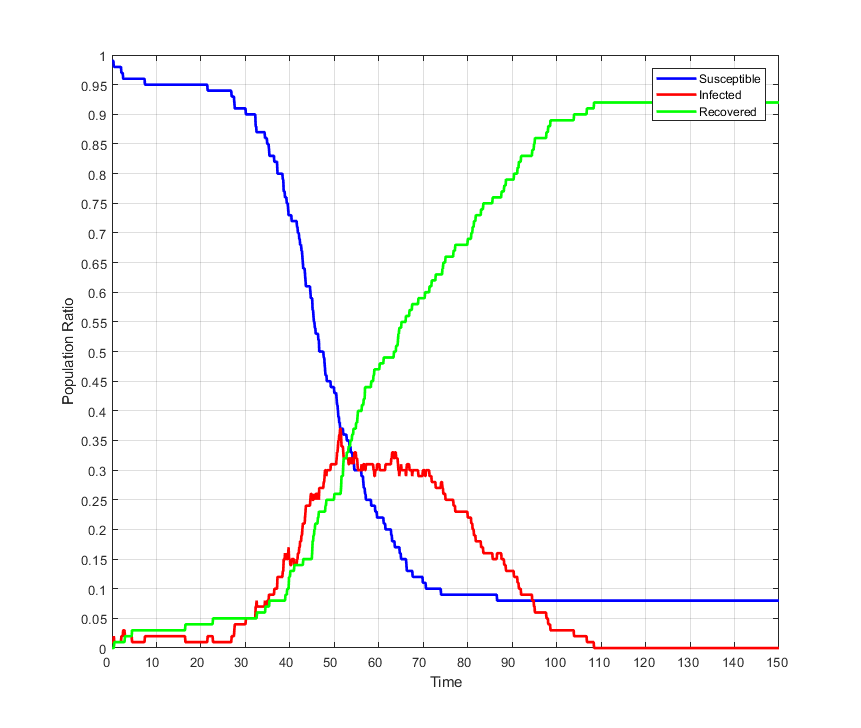
\includegraphics[width=1\textwidth, angle=0]{./fig/step2_yampa/SIR_100agents_150t_01dt.png}
			\caption{$\Delta t = 0.1$}
			\label{fig:sir_abs_approximating_01dt_100agents}
		\end{subfigure}
		
		&
    	
		\begin{subfigure}[b]{0.22\textwidth}
			\centering
			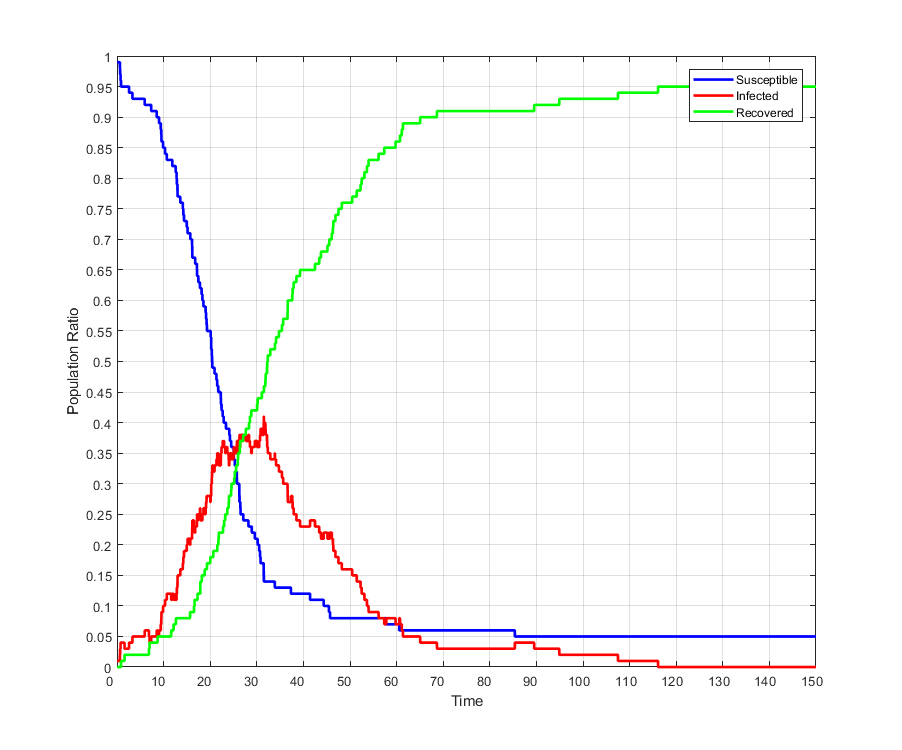
\includegraphics[width=1\textwidth, angle=0]{./fig/step2_yampa/SIR_100agents_150t_001dt.png}
			\caption{$\Delta t = 0.01$}
			\label{fig:sir_abs_approximating_001dt_500agents}
		\end{subfigure}
	\end{tabular}
	
	\caption{FRP simulation of agent-based SIR showing the influence of different $\Delta t$. Population size of 100 with contact rate $\beta = \frac{1}{5}$, infection probability $\gamma = 0.05$, illness duration $\delta = 15$ with initially 1 infected agent. Simulation run for 150 time-steps with respective $\Delta t$.} 
	\label{fig:sir_abs_dynamics_frp}
\end{center}
\end{figure}

Clearly by keeping the population size constant and just increasing the $\Delta t$ results in a closer approximation to the SD dynamics. To increasingly approximate the SD dynamics with ABS we still need a bigger population size and even smaller $\Delta t$. Unfortunately increasing both the number of agents and the sample rate results in severe performance and memory problems. A possible solution would be to implement super-sampling which would allow us to run the whole simulation with $\Delta t = 1.0$ and only sample the \textit{occasionally} function with a much higher frequency. 

\subsubsection{Discussion}
By moving on to FRP using Yampa we made a huge improvement in clarity, expressivity and robustness of our implementation. State is now implicitly encoded, depending on which signal function is active. Also by using explicit time-semantics with \textit{occasionally} we can achieve extremely fine grained stochastics. Compared to drawing a random number of events we create only a single event or none at all. This requires to sample the system with a much smaller $\Delta t$: we are treating it as a  continuous agent-based system, resulting in a hybrid SD/ABS approach.

So far we have an acceptable implementation of an agent-based SIR approach. What we are lacking at the moment is a general treatment of an environment. To conveniently introduce it we want to make use of monads which is not possible using Yampa. In the next step we make the transition to Monadic Stream Functions (MSF) as introduced in Dunai \cite{perez_functional_2016} which allows FRP within a monadic context.